\documentclass[../mech.tex]{subfiles}
\graphicspath{{\subfix{../figures/}}}
\begin{document}
\chapter{Work, Energy and Power}
\section{Translational Kinetic Energy}
An object's translational kinetic energy is given by the equation 
\[ K=\frac{1}{2}mv^2 \]
Translational kinetic energy is a scalar quantity.

Different observers may measure different values of the translational kinetic energy of an object, depending on the observer's frame of reference.
\begin{example}
    A 100 kg box shown is being pulled along the $x$-axis by a student. The box slides across a rough surface, and its position $x$ varies with time according to the equation 
    $x=0.5t^3+2t$, where $x$ is in meters and $t$ is in seconds.
    \begin{center}
        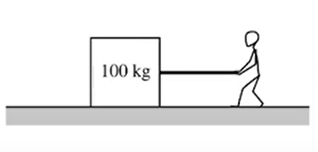
\includegraphics[width=0.5\textwidth]{3.1.PNG}
    \end{center}
    (a) Determine the speed of the box at time $t=0$.
    The derivative of the position function is $1.5t^2+2$, so $v(0)=2$ m/s 

    (b) Determine the kinetic energy of the box as a function of time.

    We know that $K=\frac{1}{2}mv^2$. Plugging in $m$ and $v$, we get $K(t)=50(1.5t^2+2)^2$.
\end{example}

\ex Two identical blocks, Block $A$ and Block $B$, slide across a horizontal surface. Block $A$ has a speed $v$, and kinetic energy $K_A$. Block $B$ has a speed 
$2v$ and a kinetic energy $K_B$. What is the ratio $K_A:K_B$ with a correct justification?

\ex \begin{center}
    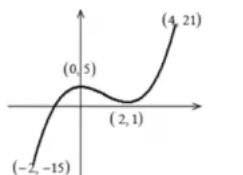
\includegraphics[width=0.5\textwidth]{3.1.1.PNG}
\end{center}
A student stands on a bus moving with a constant speed $v$ to the left as shown in Figure 1. The student $S$ is at rest relative to the bus and a ball sits at rest on the floor of the bus next to the student.
Outside the bus standing at rest relative to the ground is an observer $O$. The kinetic energies of the ball as measured by the student and the observer at this moment are $K_{S1}$ and $K_{O1}$ respectively.
As the bus passes the observer, the student kicks the ball toward the back of the bus with a constant speed less than $v$ as shown in Figure 2. The kinetic energies of the ball as measured by the student and the observer 
after the ball is kicked are $K_{S2}$ and $K_{O2}$, respectively. How do the kinetic energies measured by the student and observer compare before and after the ball is kicked?

\section{Work}
Work is the amount of energy transferred into or out of a system by a force exerted on that system over a distance.
\begin{itemize}
    \item The work done by a conservative force is path-independent and only depends on the initial and final configurations of that system.
    \item The work done by a nonconservative force is path-dependent.
\end{itemize}

Work is scalar quantity that may be positive, negative or zero.

The work done on an object by a variable force is calculated as 
\[ W=\int_a^b \vec{F}(r)\cdot \dd \vec{r} \qquad [W=Fd\cos\theta] \]
The work-energy theorem states that the change in an object's kinetic energy is equal to the sum of the work being done by all forces exerted on the object.
\[ \delta K = W \]
Work is equal to the area under the curve of a graph of $F$ as a function of displacement.
\medbreak

\begin{example}
    A skier of mass $m$ will be pulled up by a hill by a rope, as shown. The magnitude of the acceleration as a function of time $t$ can be modeled by 
    \begin{itemize}
        \item $a=a_{max}\sin \frac{\pi t}{T} (0<t<T)$
        \item $a=0 (t\geq T)$
    \end{itemize}

    Where $a_{max}$ and $T$ are constants. The hill is inclined at an angle $\theta$ above the horizontal, and friction between the skis and the snow is negligible. Express your answers in terms of given quantities and fundamental constants.
    
    \begin{center}
        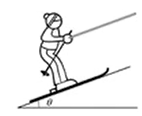
\includegraphics[width=0.5\textwidth]{3.2.PNG}
    \end{center}

    (a) Derive an expression for the velocity of the skier as a function of time during the acceleration. Assume the skier starts from rest.

    We have $v=\int a(t)\dd t = \int_0^t a_{max}\sin \frac{\pi t}{T} \dd t$,

    Integrating this and applying the limits of integration give $-\frac{a_{max}T}{\pi}\left(1-\cos\frac{\pi t}{T}\right)$ for $v$.
    \medbreak

    (b) Derive an expression for work done by the net force from the skier from rest until terminal speed is reached.

    We know $W=\Delta k$ and that $\Delta k = \frac{1}{2}mv^2$ in this case.

    Plugging in the $v$ just derived gives $W=-2a_{max}m\frac{T^2}{\pi^2}$.
\end{example}
\ex A block of mass $m$ slides with an initial velocity $v_0$ along a rough surface where the coefficient of kinetic friction between the block and the surface is $\mu$. The box comes to rest 
after sliding a distance $d_0$. A new block of unknown mass slides with an initial velocity of $2v_0$ across a surface where the coefficient of kinetic friction between the new block and the surface is $\frac{\mu}{2}$.
Write an expression that represents the distance the new block slides before coming to rest in terms of $d_0$.

\ex A force $F$ is exerted on an obejct which is initially at rest. The force varies with positions $x$ and can be described by the equation $\vec{F}=(Ax-B)\hat{i}$, where $A$ and $B$ are constants with appropriate units.
After moving a distance $D_0$, the block again comes to rest. An identical object, also initially at rest, experiences a force $2F$. The second object comes to rest again after moving a distance $D_1$. Describe the relationship between $D_0$ and $D_1$.

\section{Potential Energy}
A system composed of two or more objects has potential energy if the objects within that system only interact with each other through conservative forces.

Potential energy is a scalar quantity associated with the position of objects within a system.

The definition of zero potential energy for a given system is a decision made by the observer considering the situation to simplify or otherwise assist in analysis.

The relationship between conservative forces exerted on a system and the system's potential energy is 
\[ \delta U = -\int \vec{F}(r)\cdot \dd \vec{r} \]
The conservative forces exerted on a single dimension can be determined using the slope of a system's potential energy with respect to position in that dimension, these forces point in the direction of decreasing potential energy.
\[ F_x = -\dd u(x)/\dd x\]
The potential energy of common physical systems can be described using the physical properties of that system.

\begin{example}
    When a certain spring is stretched by an amount $x$, it produces a restoring force of $F(x)=-ax+bx^2$, where $a$ and $b$ are constants. How much work is done by an external force in stretching the spring by an amount $D$ from its equilibrium length?

    Integrate this function with bounds $0$ to $D$ to get $\frac{bD^3}{3}-\frac{aD^2}{2}$.
\end{example}

\ex The force exerted by a non-linear spring is given by $F(x)=-kx^{\left(\frac{4}{3}\right)}$. Write an expression that correctly models the potential energy stored in the spring when it is compressed a distance of $D$.

\ex \begin{center}
    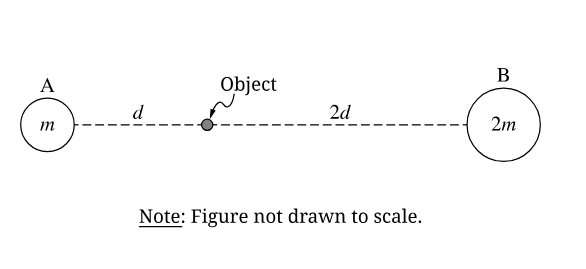
\includegraphics[width=0.5\textwidth]{3.3.PNG}
\end{center}
An object in space is placed between two planets as shown. Planet $A$ has a mass $m$ and the distance from the center of Planet $A$ to the object is $d$. Planet $B$ has a mass $2m$ and the distance 
from the center of Planet $B$ to the object is $2d$. Upon releasing the object from rest, where will the object move and how will the potential energy of the two-planet object system change?

\section{Conservation of Energy}
A system that contains objects that interact via conservative forces or that can change its shape reversibly may have both kinetic and potential energies.

Mechanical energy is the sum of a system's kinetic and potential energy.

A system may be selected so that the total energy of the system is constant.

If the total energy of a system changes, that change will be equivalent to the energy transferred into or out of the system.

Energy is conserved in all interactions.

If the work done on a selected system is zero and there are no nonconservative interactions within the system, the total mechanical energy of the system is constant.

If the work done on a selected system is nonzero, the energy is transferred between the system and the environment.

\begin{example}
    A horizontal spring with spring constant $k$ is compressed by $x$ and then used to launch a $m$ box across the floor. The coefficient of kinetic friction between the box and the floor 
    is $\mu_k$. Derive an expression for the box's launch speed $v$.

    We can determine the conservatino equation to be $-\frac{1}{2}kx^2=\frac{1}{2}mv^2+W_f$.

    $W_f=\mu mgx$, so $kx^2=mv^2+2\mu mgx$.

    Solving this equation for $v$ gives $v=\sqrt{\frac{kx^2}{m}-2\mu gx}$.
\end{example}

\ex In an experiment, an object of mass $m$ slides along a horizontal surface where friction between the object and the surface is negligible. The object has an initial speed $v$ and then collides with a spring of spring constant $k$, and the object compresses the spring a total distance 
$x$ from the equilibrium length of the spring before coming to rest. Students observing the experiment expected the object to compress the spring a distance $D$ from equilibrium, where $D>x$.
Assuming the students' expectation is correct, write an expression that can shown the change in the mechanical energy of the object-spring system during the experiment.

\ex \begin{center}
    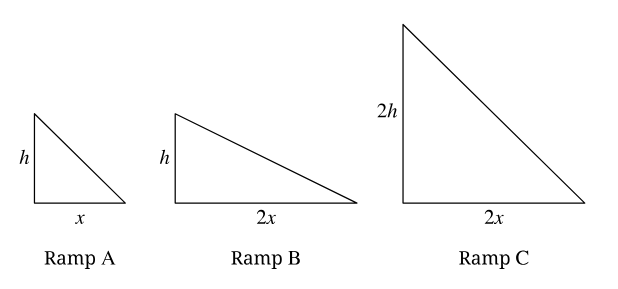
\includegraphics[width=0.5\textwidth]{3.4.PNG}
\end{center}
Three ramps, $A$, $B$, and $C$, have the dimensions shown in the figure. Identical blocks are released from rest at the top of each of the three ramps and slide to the bottom. The coefficient of kinetic friction between each of the blocks and the ramp is the same. 
Rank the speeds of the blocks at the bottom of the ramps.

\section{Power}
Power is the rate at which energy changes with respect to time, either by transfer into or out of a system or by converstion from one type to another within the system.

Average power is the amount of energy being transferred or converted, divided by the time it took for that transfer to happen.

The instantaneous power delivered to an object by a force is given by the equation:
\[ p_{ins}=\frac{\dd E}{\dd t} \]

The instantaneous power delivered to an object by the component of a constant force parallel to the object's velocity can be described with the derived equation:
\[ p_{ins}=Fv\cos\theta \]

\begin{example}
    A factory uses a motor and a cable to drag a $300$ kg machine to the proper place on the factory floor. What power must the motor supply to drag the machine at a speed of $0.50$ m/s? The coefficient of friction 
    between the machine and the floor is $0.60$.

    Let $F_{NET}=0$, so $F = \mu m g$.

    This gives us $F=1764$N.

    The power formula is $P_{ins}=F{\parallel}v = 882$W.
\end{example}

\ex A box is pushed across a surface where friction between the box and the surface is negligible. There is a resistive force from the air exerted on the box equal to $F_R=-kv$. Draw a graph that correctly models the relationship
between the power $P$ required to move the box at a constant speed $v$ to the speed of the box.

\ex \begin{center}
    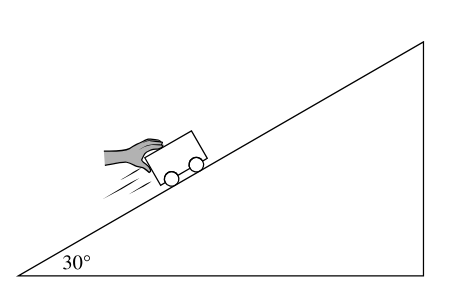
\includegraphics[width=0.5\textwidth]{3.5.PNG}
\end{center}
A $0.250$ kg cart is being pushed up a track that is inclined at $30\degree$ above the horizontal as shown. Friction between the cart and the track is negligible. Calculate the minimum power required to push the cart up the track at a constant speed of $2.4$ m/s.

\end{document}